\documentclass[ignorenonframetext,aspectratio=169,10pt,xcolor=table]{beamer}

\definecolor{EnglishViolet}{HTML}{4B3D60}
\definecolor{Crimson}{HTML}{DB162F}

\beamertemplateshadingbackground{white}{white!80!black}
\setbeamercolor{structure}{fg=EnglishViolet}
\setbeamercolor{normal text}{fg=white!25!black}
\usefonttheme{structurebold}
\setbeamercolor{footnote}{fg=gray}
\setbeamercolor{alerted text}{fg=Crimson}
\setbeamerfont{alerted text}{series=\bfseries}
\setbeamerfont{url}{series=\bfseries}
\beamertemplatenavigationsymbolsempty
\setbeamertemplate{footline}[frame number]
\setbeamertemplate{page number in head/foot}[appendixframenumber]
\setbeamertemplate{itemize items}[circle]
\hypersetup{colorlinks,linkcolor=structure,urlcolor=structure}

\usepackage[backend=biber,style=authoryear-comp]{biblatex}
\addbibresource{references.bib}
\renewbibmacro{in:}{}

\renewcommand{\footnotesize}{\tiny}

\newrobustcmd*{\footfullcitenomark}{%
  \AtNextCite{\let\thefootnote\relax\let\mkbibfootnote\mkbibfootnotetext}%
  \footfullcite%
}

\usepackage{graphicx}
\graphicspath{{figs/}}

\usepackage{tikz,pgfplots}
\usetikzlibrary{calc,shapes,positioning}
\pgfplotsset{compat=1.15}
\pgfkeys{/pgfplots/tuftelike/.style={
  semithick,
  tick style={major tick length=4pt,semithick,black},
  separate axis lines,
  axis x line*=bottom,
  axis x line shift=10pt,
  xlabel shift=5pt,
  axis y line*=left,
  axis y line shift=10pt,
  ylabel shift=5pt}}

\usepackage{menukeys}

\title{Scientific Imaging with ImageJ}
%\author{Material contributed by J\'er\^ome Boulanger, Ulrike Schlulze, Leila Mure\,san}
%\date{}

\begin{document}

\begin{frame}
  \maketitle
\end{frame}

\section{Introduction}

\begin{frame} \frametitle<presentation>{Introduction}
  The aim of this session is to learn:

  ~~

  \begin{itemize}   \setlength\itemsep{1em}
    \item How to improve handling of scientific images for quantification and
      illustation,
    \item Understand core concepts about images,
    \item Discover ImageJ/Fiji,
    \item Know where to look for information,
    \item Discover a few useful plugins,
    \item Acquire good practices.
  \end{itemize}
\end{frame}


\begin{frame} \frametitle{Context}
  \begin{block}{Quantification}
    \begin{itemize}
    \item Measure objects properties (intensity, area, shape, \dots)
    \item Count objects
    \item Relationship (co-occurrence, co-localisation), hierarchical.
    \item Speed, motion, \dots
    \end{itemize}
  \end{block}
  \begin{block}{Illustration}

    \begin{itemize}
    \item Use ImageJ to prepare the elements of a figure and import
      them in Illustrator.
    \item Relationship between markers
    \item Localisation of organelles
    \item Scale of objects
    \end{itemize}
  \end{block}
\end{frame}


\begin{frame} \frametitle{The ImageJ software}

  \begin{center}
    \includegraphics[width=0.5\textwidth]{ij}
  \end{center}

  \begin{itemize}  \setlength\itemsep{1em}
  \item ImageJ is a Java based image processing software.
  \item Java programs run on the java virtual machine (JVM)
  \item Can run on many operating system (Microsoft Windows, Mac OS,
    Linux, \dots)
  \item Developed by Wayne Rasband since 1997 at the National
    Institute of Health
  \item ImageJ eco-system
    \begin{itemize}
    \item ImageJ2: rewrite of ImageJ for multi dimensional data
    \item Fiji: image processing package built around ImageJ2
    \end{itemize}
  \end{itemize}

  \footfullcitenomark{ij2}
  \footfullcitenomark{schneider_nih_2012}

\end{frame}


\begin{frame} \frametitle{Installation \& Updating}

  \begin{block}{First Installation}
    \begin{itemize}
    \item Download Fiji from  \url{https://imagej.net/software/fiji/downloads}.
    \item For windows:
    \begin{itemize}
      \item Unzip and save somewhere on your hard drive where default
      users have access (not C:\\Program Files).
      \item Open the folder and double click on ImageJ-win64
      and create a shortcut.
    \end{itemize}
    \item MacOS: 
    \begin{itemize}
      \item Move Fiji.app from the "Downloads" folder to the "Applications" folder
     \item Open the security setting, find Fiji was blocked and click open anyway button.
    \end{itemize}
    \end{itemize}
  \end{block}

  \begin{block}{Updating}
    \begin{itemize}
    \item To update ImageJ to the latest version \menu{Help > Update
        ImageJ}.
    \item To install/update plugins collections and manage update
      sites \menu{Help > Update}
    \end{itemize}
  \end{block}

\end{frame}

\begin{frame}  \frametitle{Fiji.app folder content}

  The Fiji.app folder is organized into several subfolders:

  \begin{itemize} \setlength\itemsep{1em}
  \item \directory{jars}: contains the main jar (eg ij-1.53q.jar) and
    extra java dependencies
  \item \directory{macros}: contains macros you installed and the
    \texttt{StartupMacros.fiji.ijm}
  \item \directory{plugins}: contains the jar (java artifacts) of the
    plugins
  \item \directory{scripts}: contains a few matlab scripts
  \item \directory{lut}: look up tables (mapping for intensity to displayed
    colors)
  \end{itemize}

\end{frame}


\begin{frame} \frametitle{Image is data}

  \begin{columns}
    \begin{column}{.5\textwidth}
      For point scanner or camera based imaging systems:
      \begin{itemize} \setlength\itemsep{1em}
      \item Sensors converts the number of detected photo-electrons
        into an electric voltage
      \item This voltage is then digitized into a number by the A/D
        converter.
      \item The image can be seen as an array of values with columns
        $x$ and rows $y$ starting in the top left corner with coordinates $(0,0)$.
      \end{itemize}
      \end{column}

    \begin{column}{.5\textwidth}
      \only<1>{
        \begin{tikzpicture}
          \begin{axis}[name=plot1,width=5.5cm,height=4.45cm,axis on
              top, enlargelimits=false, y dir = reverse, xlabel=x,ylabel=y] \addplot
            graphics[xmin=00,xmax=600,ymin=500,ymax=0] {array_img}; \draw[red,very
              thick] (axis cs:178,231) rectangle (axis cs:202,255);
          \end{axis}
        \end{tikzpicture}
      }
      \only<2>{\includegraphics[width=.9\textwidth]{array_pixels}}
    \end{column}

  \end{columns}

\end{frame}

\begin{frame} \frametitle{A good image is good data}
  Some experimental decisions can help the downstream image analysis, eg:
  \begin{itemize}
    \item Match the microscope setting to your experiment (objective, sampling, 3D, timelapse \dots)
    \item Add house keeping labels (DAPI/Hoechst, WGA, etc) independent of you variables of interest
    \item Be aware of possible cross talk (https://www.fpbase.org/) between channels
    \item Do you want a readout per cell or per field of view?
    \item Is the spatial context important (large field of view/tiling necessary)
  \end{itemize}
\end{frame}

\begin{frame} \frametitle{General image formats}

  \begin{columns}

    \begin{column}{0.75\textwidth}
      \begin{itemize} \setlength\itemsep{1em}
      \item Digital images can be saved from the volatile memory (RAM)
        of a computer to its persistent memory (HDD/SSD) as files with various
        formats.
      \item Most file formats include some sort of compression:
        \begin{itemize}
        \item Lossless compression (PNG): original values can be
          exactly retreived
        \item Lossy compression (JPEG): information is lost when
          storing the image
        \item Both (TIF): some formats are containers which can
          include various type of compression
        \end{itemize}
      \item ImageJ can read and write natively a few format such as
        TIFF, PNG, JPG
      \item Use TIF for saving intermediate results (with/without LZW
        compression) and PNG for figures
      \end{itemize}
    \end{column}

    \begin{column}{0.25\textwidth}
      \includegraphics[width=\textwidth]{drive}
    \end{column}

  \end{columns}

\end{frame}

\begin{frame} \frametitle{Microscope vendor image formats}

  \begin{itemize}
    \item Zeiss
      \begin{itemize} \setlength\itemsep{1em}
      \item LSM: TIF based file format with additional metadata and LZW
        compression
      \item CZI: JPEG-XR and Zstd lossless compressed image
      \end{itemize}
    \item Nikon
      \begin{itemize}
        \item ND2: JPEG-2000 lossless compression
      \end{itemize}
    \item Leica
      \begin{itemize}
        \item LIF: document with several images
      \end{itemize}
    \item Olympus/Evident
      \begin{itemize}
        \item OIF: multi file formats with associated images in a folder
        \item OIB: store multiple OIF and dependent image in one file
        \item VSI: store data as a pyramid for fast visualization (.vsi/.ets)
      \end{itemize}
  \end{itemize}

  Fiji uses \href{https://imagej.net/formats/bio-formats}{bioformats} to load these files (installed by default).

\end{frame}


\begin{frame} \frametitle{Metadata}

  \begin {itemize} \setlength\itemsep{1em}
    \item Metadata are essential to the interpretation and processing of
      the image
    \item Acquisition software collect additional information that are
      stored in the files
    \begin{itemize}
      \item Pixel size in x, y, z
      \item Detectors
      \item Objective
      \item Emission wavelength
      \item \dots
     \end{itemize}
    \item The Open Microscopy Environment (OME) defines a specification
    for storing data on biological imaging.
  \end{itemize}

  \footfullcitenomark{ome-schema}
  \footfullcitenomark{fair}
  \footfullcitenomark{linkert_metadata_2010}

\end{frame}

\begin{frame} \frametitle{Loading an image}
  \begin{itemize} \setlength\itemsep{2em}
  \item Fiji will detect supported file format when selecting
    \menu{File>Open} and use bioformat if needed to load an image from
    disk to memory.
  \item You can also use \menu{Plugins > Bio-Formats > Bio-Formats
      Importer} to use Bio-formats directly
  \item The Bio-Formats plugin remember previous settings, so use
    the tool directly to define the way the drag and drop or
    \menu{File>Open} behaves on non-native formats.
  \end{itemize}
\end{frame}

\begin{frame} \frametitle{Pixel size calibration \& scale bar}

  \begin{columns}

    \begin{column}{0.5\textwidth}
      \begin{itemize} \setlength\itemsep{1em}
      \item Use \menu{Image>Properties\dots} to check and set the
        pixel size in each dimensions
      \item Use \menu{Analyze>Set Scale\dots} to use an known distance
        to set the scale
      \item Use \menu{Analyze>Tools>Scale Bar} to display the scale on
        a calibrated image
      \item Saving the image as TIF will encode the pixel calibration, other
      formats (PNG, JPEG) will loose it.
      \end{itemize}
    \end{column}

    \begin{column}{0.5\textwidth}
      \includegraphics[width=\textwidth]{clown-scale}
    \end{column}

  \end{columns}

\end{frame}

\begin{frame} \frametitle{Quantization}

  \begin{columns}

    \begin{column}{0.7\textwidth}
      \begin{itemize} \setlength\itemsep{1em}
      \item The intensity values are quantized into grey levels
      \item Images are saved as 8-bit or 16-bit images by acquisition
        software.
        \begin{itemize}
        \item For camera sensor (CCD, CMOS), photo-electron are
          accumulated in wells and converted into analogue voltages that are
          then digitized. Well depth is in the order of ~40000 electrons.
        \item For photo-multiplier tubes (PMT) photo-electrons are
          amplified using a chain of dynodes enabling to count individual
          photons. Number of photon is low ($\leq 255$).
        \end{itemize}
      \end{itemize}
      \begin{itemize}
      \item Use \menu{Image>Type>8-bit} to check \& convert an image
        to 8-bit, using the current dynamic range.
      \item Converting to lower bit depth may result in loss of information.
      \end{itemize}
    \end{column}

    \begin{column}{0.3\textwidth}
      \begin{center} \small \rowcolors{1}{gray!25!bg}{white!25!bg}
        \begin{tabular}{cl}
          Bit depth & Dynamic range \\ \hline 8 &
          0-255 \\ 12 & 0-4095\\ 14 & 0-16383\\ 16 & 0-65535
        \end{tabular}
      \end{center}

    \end{column}

  \end{columns}

\end{frame}

\begin{frame} \frametitle{Brightness \& Contrast adjustment}

  \begin{itemize}\setlength\itemsep{1em}
    \item \menu{Image > Adjust > Brightness \& Contrast...} or
      \keys{\Alt+\shift+C} launches the B\&C tool
    \item Pixels intensities are mapped linearly to the displayed
      intensity.
    \item Enable to discard unused part of the dynamic range
    \item Adjust the Minimum and Maximum of the dynamic range which will
      be displayed.
    \item Adjust the Brightness and Contrast to change how they are
      display.
    \item Press \menu{Auto} to stretch the intensities between a
      predefined percentage of saturated pixels. Equivalent to \menu{Process
        > Enhance Contrast...} with the normalized option left unticked.
    \item Press \menu{Apply} to change the pixel values.
    \item When changing the image mode (16-bit to 8-bit or 32-bit to
      8-bit) the B\&C settings are applied to the image.
  \end{itemize}

\end{frame}


\begin{frame} \frametitle{Histogram}

  \begin{columns}

    \begin{column}{0.5\textwidth}
      \begin{itemize}\setlength\itemsep{1em}
      \item Shows the frequency of each intensity values
      \item Use \menu{Analyze>Histogram} or \keys{\ctrl+h} to display the
        histogram
      \item Helps identify clipped values (under/over exposed, saturated)
      \item Visualise classes of pixels
      \item Good for detecting manipulated images
      \end{itemize}
    \end{column}

    \begin{column}{0.5\textwidth}
      \begin{center}
        \includegraphics[width=\textwidth]{histogram}

        {\tiny ImageJ histogram}
      \end{center}
    \end{column}

  \end{columns}

\end{frame}

\begin{frame} \frametitle{Look up table (LUT)}

  \begin{columns}

    \begin{column}{0.6\textwidth}
      \begin{itemize} \setlength\itemsep{1em}
      \item Intensities are mapped to a color defined by a red, green
        and blue triplet value for display.
      \item Converting an image to RGB applies the current LUT
        (\menu{Apply LUT} taking into account the B\&C settings)
      \item LUT can be inverted (black becomes white, \dots)
      \item Use LUT to help people with colour blindness.
      \item You quickly access LUT tools from the toolbar.
      \end{itemize}
    \end{column}

    \begin{column}{0.4\textwidth}
      \begin{center}
        \begin{tikzpicture}
          \begin{axis}[
              width=5cm,
              height=4cm,
              xlabel=Intensity,
              ylabel=Color,
              domain=0:255,
              axis x line=center,
              axis y line=center]
            \shade[left color=black,right color=white] (axis cs:0,0) rectangle (axis cs: 255,10);
            \shade[bottom color=blue,top color=red] (axis cs:0,0) rectangle (axis cs: 10,255);
            \addplot[structure,thick]{x}; \draw[thick,->] (128,15) -- (128,120);
            \draw[thick,->] (120,128) -- (15,128);
          \end{axis}
        \end{tikzpicture}

        {\tiny Intensity to color mapping}

        ~~

        \includegraphics[width=\textwidth]{lut-tools.png}

        {\tiny ImageJ LUT toolbar}
      \end{center}
    \end{column}

  \end{columns}

\end{frame}


\begin{frame} \frametitle{Multi-channel images}

  \begin{itemize} \setlength\itemsep{1em}
    \item Multi-channel images can be easily acquired by microcopes
      (multiple wavelength/fluorophores, brightfield/DIC, \dots)
    \item There are two types of color images:
      \begin{itemize}
      \item RGB images store color information into a single ($8 \times
        3$) 24 bit image
      \item Composite image are image whose channels are stored as
        individual (8,16-32-bit) image planes
      \end{itemize}
    \item On a composite image use \menu{Image>Color>Channel Tool} or
      \keys{\ctrl+\shift+z} to select the channel to display
    \item Create a multi channel image using \menu{Image>Color>Merge
        Channels\dots}
    \item Split channels of an image using \menu{Image>Color>Split
        Channels}
  \end{itemize}

\end{frame}


\begin{frame} \frametitle{Multi-dimensional images}
  \framesubtitle{Stack \& Hyperstacks}
  \begin{itemize} \setlength\itemsep{1em}
    \item Images can have many dimensions (axis) associated to them
      channel c, time t, depth.
    \item Image stacks represent up to 4 dimensions (xyzc or xytc) with
      a maximum of 3 channels.
    \item Hyperstacks can have up to 5 dimensions xyzct with no limits
      on the number of channels.
    \item Virtual stacks enable to load only the images planes which are
      visualised.
  \end{itemize}

  To quickly visualize multi-dimensional data, use :

  \begin{itemize}
    \item Orthogonal views (\menu{Image>Stack>Orthogonal Views}) or
      \keys{\ctrl+\shift+H} can help visualize 3D data
    \item Maximum intensity projection \menu{Image>Stack>Z Project\dots}
    \item Reslice a stack with \menu{Image>Stack>Reslice\dots} or press \keys{/}
    \item To synchronize two stacks use \menu{Analyze>Tools>Synchronize Windows}
  \end{itemize}
\end{frame}


\begin{frame} \frametitle{Basic manipulation}

  \begin{itemize} \setlength\itemsep{1.5em}
    \item Duplicate \keys{\ctrl+\shift+D} allows to crop, select
      channels and slices
    \item Use \keys{{+}} and \keys{-} or the magnifying glass tool to zoom
      in and out the displayed image.
    \item Use the hand tool to pan within a zoomed image.
    \item Changing the actual pixel size:
      \begin{itemize}
      \item \menu{Image>Scale} scale the image, if ``create a new
        image'' is not ticked, the image keep the same number of pixels and is
        cropped or padded as necessary.
      \item \menu{Image>Adjust>Size\dots} scale the image in place
        without cropping or creating a new image.
      \end{itemize}
    \item Use the search bar to look for tools.
  \end{itemize}

\end{frame}

\begin{frame} \frametitle{Background correction}

  \begin{columns}
    \begin{column}{0.6\textwidth}
      \begin{itemize} \setlength\itemsep{1em}
      \item Uneven background makes images difficult to segment using a threshold.
      \item Background level can vary for several reason:
        \begin{itemize}
        \item Uneven illumination
        \item Scattering
        \item Auto fluorescence
        \end{itemize}
      \item We can apply a few generic correction, to help thresholding the image
        \begin{itemize}
        \item Rolling ball from \menu{Process>Subtract Background\dots}
        \item Top Hat (image - grayscale opening) from
          \menu{Process>Filter>Top Hat\dots}
        \end{itemize}
      \item Note that the resulting intensity remains hard to compare at different
        location within the image.
      \end{itemize}
    \end{column}

    \begin{column}{0.4\textwidth}
      \begin{center}
        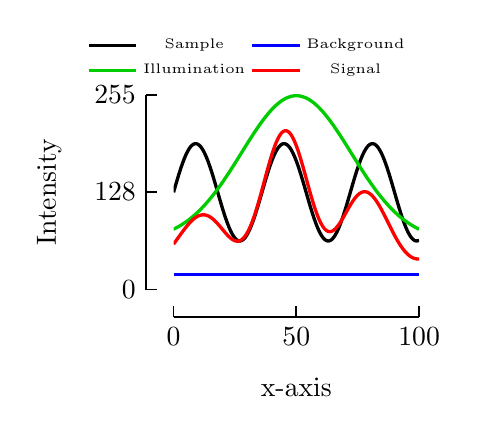
\begin{tikzpicture}

          \begin{axis}[tuftelike,
              domain=0:100,
              samples=200,
              no markers,
              ymin=0,ymax=255,xmin=0,xmax=100,
              xlabel={x-axis},ylabel=Intensity,
              width=4.7cm,
              ytick={0,128,255},xtick={0,50,100},
              legend style={at={(1,1.35)},legend columns=2,fill=none,draw=none,font=\tiny}]

            \addplot[very thick,black] {255*(0.5+0.25*sin(10*x)};
            \addlegendentry{Sample}
            \addplot[very thick,blue] {20};
            \addlegendentry{Background}
            \addplot[very thick,green!80!black] {254*(0.25+0.75*exp(-0.001*(x-50)*(x-50)))};
            \addlegendentry{Illumination}
            \addplot[very thick,red] {20 + 255*(0.5+0.25*sin(10*x)) * (0.25+0.75*exp(-0.001*(x-50)*(x-50)))};
            \addlegendentry{Signal}

          \end{axis}

        \end{tikzpicture}

      {\tiny Uneven illumination}
    \end{center}

    \end{column}

  \end{columns}

\end{frame}


\begin{frame} \frametitle{Filtering}

  Image filtering can help reduce noise and is useful as a preprocessing to
  obtain smooth outline.

  \begin{itemize} \setlength\itemsep{1em}
    \item Box filtering \keys{\ctrl+\shift+S}
    \item Gaussian filtering \menu{Process>Filters>Gaussian Blur\dots}
    \item Median filtering \menu{Process>Filters>Gaussian Blur\dots}
  \end{itemize}

  \begin{center}
    \begin{tabular}{ c c c c}
      Original & Smooth & Gaussian 5px  & Median 2px\\
      \includegraphics[width=0.2\textwidth]{flt-original}&
      \includegraphics[width=0.2\textwidth]{flt-smooth}&
      \includegraphics[width=0.2\textwidth]{flt-gaussian5}&
      \includegraphics[width=0.2\textwidth]{flt-median2}
    \end{tabular}
  \end{center}

\end{frame}


\begin{frame} \frametitle{Selection / Region Of Interest (ROI)}

  \begin{itemize} \setlength\itemsep{1em}
    \item Use the rectangle, circle, polygon, freehand, line tools to
      create selections.
    \item Use \menu{Edit>Selection>Specify} to enter manually the
      coordinate of a shape
    \item Transfer selection across images using
      \menu{Edit>Selection>Restore Selection} or \keys{\ctrl+\shift+E}
    \item Store selection into the ROI manager \menu{Edit>Selection>Add
        to manager} or \keys{t}
    \item Use \menu{Edit>Selection>Select None} \keys{\ctrl+\shift+A} to
      be sure no selection is active
    \item ROI from the ROI Manager can be stored as individual
      proprietary .roi file or as a collection into a .zip file.
    \item ROIs can be combined together using AND, OR, XOR logical
      operation
    \item Use \menu{Edit>Draw} and \menu{Edit>Fill} to set the pixel
      values on the contours resp. the inside of the shape to the value
      define by the colour picker tool.
  \end{itemize}

\end{frame}


\begin{frame} \frametitle{Threshold}
  \begin{columns}
    \begin{column}{0.7\textwidth}
      \begin{itemize} \setlength\itemsep{1em}
      \item Thresholding an image gives a binary image: 8-bit image with
        values either "True" (0) or "False" (255).
      \item Use the sort cut \keys{ctrl+\shift+T} to display the threshold
        tool.
        \begin{itemize}
        \item Use the sliders to set the upper and lower values
        \item Auto thresholds: Fiji includes a set of automatic threshold
          \url{https://imagej.net/plugins/auto-threshold}
        \item Stack histogram: the statistics will be computed on the all
          stack
        \end{itemize}
      \item Use \menu{Apply} or \menu{Process>Binary>Convert to mask} to
        apply the threshold and make the image binary.
      \item The menu \menu{Process>Binary>Make binary} will show a dialog
        if a threshold has been set.
      \item The LUT of binary images is inverted
      \end{itemize}
    \end{column}
    \begin{column}{0.3\textwidth} \centering
      \includegraphics[width=\textwidth]{threshold}
    \end{column}
  \end{columns}
\end{frame}

\begin{frame} \frametitle{Binary image processing}

  \begin{itemize} \setlength\itemsep{1em}
  \item \menu{Process>Binary>Dilate} grow the masks, similar to
    \menu{Process>Filter>Maximum\dots}
  \item \menu{Process>Binary>Erode} shrink the masks, similar to
    \menu{Process>Filter>Minimum\dots}
  \item \menu{Process>Binary>Open} is equivalent to erode followed by
    dilate, removes small objects and lines
  \item \menu{Process>Binary>Close-} is equivalent to dilate followed
    by erode, bridge non touching objects etc
  \item \menu{Process>Binary>Watershed} separate touching objects
  \item \menu{Process>Binary>Fill Holes} will fill holes in the masks
  \end{itemize}
  \begin{center} \includegraphics[width=\textwidth]{flower}
  \end{center}
\end{frame}


\begin{frame} \frametitle{From thresholds to regions of interests}
    \begin{columns}
      \begin{column}{0.5\textwidth}
    \begin{itemize}
    \item Use \menu{Edit>Selection>Create selection} to convert the
      threshold to a selection (can be a composite selection).
      \begin{center}
      \includegraphics[width=0.7\textwidth]{threshold2selection}
      \end{center}
    \end{itemize}
  \end{column}
  \begin{column}{0.5\textwidth}
    \begin{itemize}
      \item Use the \menu{Analyze>Analyze Particles\dots} to convert
      connected components into individual ROIs and add them to the ROI
      Manager.
      \begin{center}
        \includegraphics[width=0.7\textwidth]{thresholdroimanager}
      \end{center}
    \end{itemize}
  \end{column}
  \end{columns}
\end{frame}


\begin{frame} \frametitle{Measurements}
  \begin{columns}
    \begin{column}{0.65\textwidth}
      \begin{itemize} \setlength\itemsep{2em}
      \item Use \menu{Analyze>Set Measurements} to define the
        quantity to be measured
      \item Select an individual ROI and press \keys{\ctrl+M} to add
        measurements to the Result table.
      \item To measure the properties of all ROI stored in the ROI
        Manager, select them all with \keys{\ctrl+A} and press \menu{Measure}
      \end{itemize}
    \end{column}
    \begin{column}{0.35\textwidth}
      \includegraphics[width=\textwidth]{measure}
    \end{column}
  \end{columns}
\end{frame}

\begin{frame} \frametitle{Advanced morphological operation}
  \begin{columns}
    \begin{column}{0.65\textwidth}
  MorpholibJ provides additional morphological operations in 2D and 3D.
  \begin{block}{Installation}
    \begin{itemize}
    \item Activate the IJPB-plugins update site
    \end{itemize}
  \end{block}
  \begin{block}{Example usage}
    \begin{itemize}
      \item 3D morphological operations
      \item Label connected components
      \item Size filtering
      \item Seeded watershed
      \end{itemize}
  \end{block}
\end{column}
\begin{column}{0.35\textwidth}
  \includegraphics[width=\textwidth]{seeded_watershed}
\end{column}
\end{columns}
\end{frame}


\begin{frame} \frametitle{Co-localization}
  There are several types of colocalization
  \begin{itemize}
    \item correlation coefficients: Pearson correlation coefficient
    \item overlap  coefficients: Manders coefficients
    \item point base colocalization
  \end{itemize}

\end{frame}

% \begin{frame} \frametitle{Affine stabilization}
%   Image registration aims at aligning two images to each other.

%   \begin{block}{Installation}
%     \begin{itemize}
%     \item Activate the BIG_EPFL and MultiStackReg update site
%     \end{itemize}
%   \end{block}

%   \begin{block}{Usage}
%     \begin{itemize}
%     \item Select the motion model: translation, rigid, scaled rotation or affine
%     \item Use MultiStackReg, to register more than one stack
%     \end{itemize}
%   \end{block}
% \end{frame}


% \begin{frame} \frametitle{Particle tracking with TrackMate}
%   \begin{enumerate}
%   \item Trackmate is 
%   \item Linking the successive position of object over time
%   \item Enable to extract speed, intensity variation, etc over time
%   \end{enumerate}
%   \begin{block}{Usage}
%     \begin{itemize}
%     \item Select a detector and adjust its parameters
%     \item 
%     \end{itemize}
%   \end{block}
% \end{frame}

% \begin{frame} \frametitle{Pixel classification with Labkit}

% \end{frame}

\begin{frame} \frametitle{Stardist}

  \begin{block}{Installation}
    \begin{itemize}
    \item Activate the CSBDeep and the Stardist update sites
    \end{itemize}
  \end{block}
  \begin{block}{Usage}
    \begin{itemize}
    \item Startdist is neural network for star convex polygon segmentation.
    \item Pre-trained weights can be loaded for nuclei segmentation.
    \end{itemize}
    \begin{center}
      \includegraphics[width=0.75\textwidth]{stardist}
    \end{center}
  \end{block}

  \centering
  \footfullcitenomark{stardist}

\end{frame}

\begin{frame} \frametitle{Creating a workflow}

  \begin{block}{Building a workflow}
    An analysis can have the following typical steps:
    \begin{itemize}
      \item Duplicate
      \item Pre-process (background substraction, filtering)
      \item Threshold
      \item Process binary masks
      \item Populate the ROI manager
      \item Perform measurements on the original image
    \end{itemize}
  \end{block}

  \begin{block}{Recording and scripting}
    Recording and scripting allows to reproduce the workflow on other images.
  \end{block}

\end{frame}


\begin{frame} \frametitle{Image integrity}

  \begin{itemize}
  \item Apply adjustments to the entire image
  \item Track the sequence of manipulations (scripts/macro)
  \end{itemize}

  Include in the legend or methods section the following
  information:
  \begin{itemize}\small

  \item Equipment (microscopes, lenses, cameras, detectors,
    filters, software).

     \begin{itemize}
     \item[bad] Pictures were taken on the Zeiss\_780\_2S370.
     \item[good] Images acquired on a Zeiss LSM 780 inverted
    microscope controlled by Zen black and equiped with a 63x/1.4 oil
    objective using a 488nm laser and GaAsp detectors.
     \end{itemize}

  \item Time and space sampling (pixel size), image bit depth,
    temperature, imaging medium, fluorochromes
  \item Look up table, gamma correction
  \item Processing software and manipulations: deconvolution, 3D reconstructions,
   volume rendering, filtering, nonlinear operation, thresholding and projection
  \end{itemize}

  \footfullcitenomark{nature-figs}
  \footfullcitenomark{ori-guidelines}
  \footfullcitenomark{noauthor_image_2010}

\end{frame}


\begin{frame}{The FAIR Guiding Principles}
  \begin{columns} \small
    \begin{column}{0.5\textwidth}
  \begin{block}{Findable}
    \begin{itemize}
    \item (meta)data are assigned a globally unique and persistent identifier
    \item data are described with rich metadata 
    \item metadata clearly and explicitly include the identifier of the data it describes
    \item (meta)data are registered or indexed in a searchable resource
    \end{itemize}
  \end{block}

  \begin{block}{Accessible}
    \begin{itemize}
    \item (meta)data are retrievable by their identifier using a standardized protocol
      \begin{itemize}
      \item  open, free, and universally implementable
      \item  allows for an authentication and authorization procedure
      \end{itemize}
    \item metadata are accessible, even when the data are no longer available
    \end{itemize}
  \end{block}
\end{column}
  \begin{column}{0.5\textwidth}
  \begin{block}{Interoperable}
    \begin{itemize}
    \item (meta)data use a formal, accessible, shared, and broadly applicable language for knowledge representation.
    \item (meta)data include qualified references to other (meta)data
    \end{itemize}
  \end{block}

    \begin{block}{Reusable}
      \begin{itemize}
      \item meta(data) are richly described with a plurality of accurate and relevant attributes
        \begin{itemize}
        \item (meta)data are released with a clear and accessible data usage license
        \item (meta)data are associated with detailed provenance
        \item (meta)data meet domain-relevant community standards
        \end{itemize}
      \end{itemize}
    \end{block}
  \end{column}
  \end{columns}
    \footfullcitenomark{fair}
    \footfullcitenomark{cambridge-dmp}

  \end{frame}


\begin{frame} \frametitle{Data repository}

  Publicly accessible dataset increase the number of citation of published
  articles \footfullcite{colavizza_citation_2020}.

  \begin{block}{Image Data Repository \url{https://idr.openmicroscopy.org}}
    Public repository of image datasets from published scientific studies, where
    the community can submit, search and access high-quality bio-image data.
    Supported by BBSRC, Wellcome Trust and EBI. Dedicated viewer for microscopy data.
  \end{block}

  \begin{block}{Zenodo \url{https://zenodo.org}}
    General-purpose open repository supported by CERN. Associate a citable doi
    to digital assets.
  \end{block}

  \begin{block}{Figshare \url{https://figshare.com}}
    Upload up to 20GB of data and share privatly, publish (doi)
  \end{block}

  \begin{block}{DRYAD \url{https://datadryad.org}}
    Curated resource that makes research data discoverable, freely reusable, and citable.
  \end{block}

  \footfullcitenomark{idr}
  \footfullcitenomark{plosone-opendata}
  \footfullcitenomark{cambridge-datamanagment}

\end{frame}

%% Additional information
% \begin{frame}{Data Repositories}
%   \begin{itemize}
%     \item IDR ( \url{idr.openmicroscopy.org})
%     \item Zenodo ( \url{zenodo.org})
%     \item Mendeley Data ( \url{data.mendeley.com})
%     \item DataHub ( \url{datahub.io})
%     \item FigShare ( \url{figshare.com})
%   \end{itemize}

%   ~~

%   More info:
%   \begin{itemize} \tiny
%     \item \url{https://www.ukri.org/about-us/mrc/our-policies-and-standards/research/data-management-and-sharing/}
%     \item \url{https://osc.cam.ac.uk/open-research/data-management-sharing},
%     \item \url{https://www.data.cam.ac.uk},
%     \item \url{https://plos.org/open-science/open-data}
%   \end{itemize}

%   \end{frame}

%% \begin{frame}{Software good practice}
%% \begin{itemize}
%% 	\item Use meaningful variable and function names
%% 	\item Write comments, documentation. Provide usage examples.
%% 	\item Use a publicly accessible repository with version control. \\
%% 	 (GitHub, GitLab,Bitbucket...). Add a license.\\
%% 	It helps:
%% 	\begin{itemize}
%% 	\item to track changes in your software
%% 	\item collaborations
%% 	\item reproducibility of results
%% 	\item reusability
%% 	\item to improves software quality.
%% 	\end{itemize}
%% 	\item Register code in a community registry, making it easy to find
%% 	\item Enable citation of the software
%% 	\item Use a software quality checklist
%% \end{itemize}
%% \begin{flushright}
%% {\tiny \url{https://fair-software.eu}}
%% \end{flushright}
%% \end{frame}

\begin{frame} \frametitle{ImageJ Cheatsheet}

  \begin{columns}

    \begin{column}{0.5\textwidth}
      \begin{tabular}{ll}
        Image properties &\keys{\ctrl+\shift+P} \\
        Duplicate/crop & \keys{\ctrl+\shift+D} \\
        BrightnessContrast & \keys{\Alt+\shift+C} \\
        Channel Tools & \keys{\ctrl+\shift+Z} \\
        Add to ROI Manager & \keys{t} \\
        Restore Selection & \keys{\ctrl+\shift+E} \\
        Select All & \keys{\ctrl+A} \\
        Select None & \keys{\ctrl+\shift+A}\\
      \end{tabular}
    \end{column}

    \begin{column}{0.5\textwidth}
      \begin{tabular}{ll}
        Histogram & \keys{\ctrl+H} \\
        Orthoslices & \keys{\ctrl+\shift+H}\\
        Reslice & \keys{/} \\
        Threshold & \keys{ctrl+\shift+T} \\
        Measure & \keys{\ctrl+M} \\
        Smooth & \keys{\ctrl+\shift+S} \\
        Plot profile & \keys{\ctrl+K} \\
      \end{tabular}
    \end{column}

  \end{columns}

\end{frame}


\begin{frame}{Online ressources}
  \begin{itemize}
    \item \url{https://imagej.net}
    \item \url{https://forum.image.sc}
  \end{itemize}
\end{frame}

\end{document}